\input ../SlidePreamble
\input ../preamble

\begin{document}

{\Huge

  \centerline{\bf TTIC 31230, Fundamentals of Deep Learning}
  \bigskip
  \centerline{David McAllester, Winter 2020}
  \vfill
  \centerline{\bf Language Modeling}

\slide{Natural Language Understanding}

GLUE: General Language Understanding Evaluation

\vfill

\centerline{\normalsize ArXiv 1804.07461}
\centerline{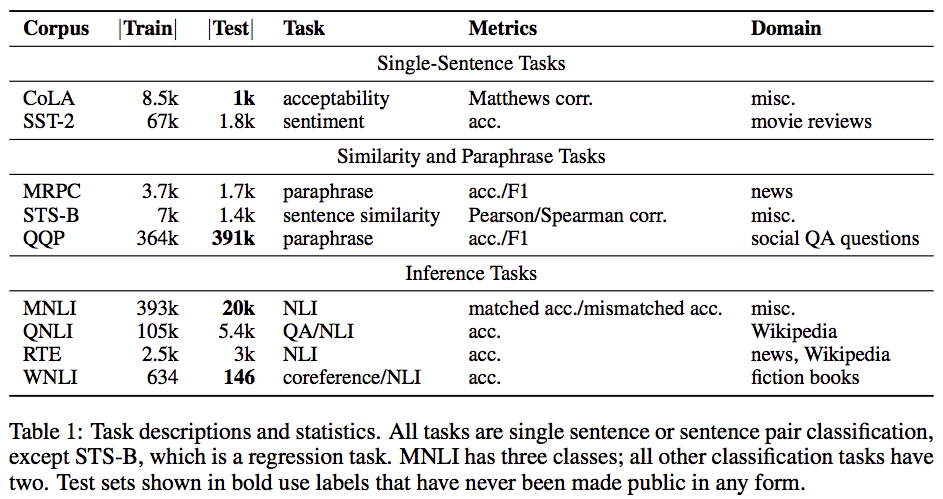
\includegraphics[width= 7in]{\images/GLUE}}

\slide{BERT and GLUE}

\centerline{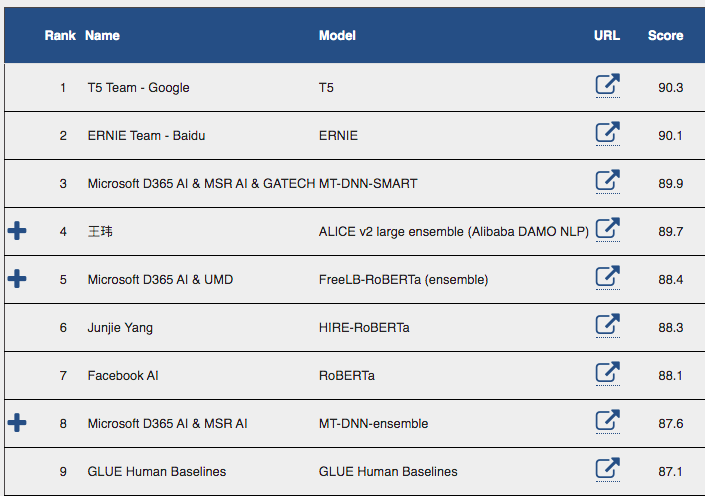
\includegraphics[width= 7in]{\images/GLUELeader}}

\slide{BERT and SuperGLUE}

\centerline{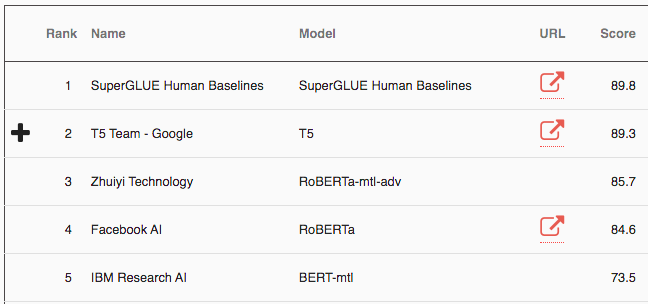
\includegraphics[width= 9in]{\images/SuperLeader}}

\slide{Language Modeling}

The recent progress on NLP benchmarks is due to pretraining on language modeling.

\vfill
Langauge modeling is based on unconditional cross-entropy minimiztion.

\vfill
$$\Phi^* = \argmin_\Phi \;E_{y \sim \pop}\;-\ln P_\Phi(y)$$

\vfill
In language modeling $y$ is a sentence (or fixed length block of text).

\slide{Language Modeling}

Let $W$ be some finite vocabulary of tokens (words).

\vfill
Let $\mathrm{Pop}$ be a population distribution over $W^*$ (sentences).

\vfill
We want to train a model $P_\Phi(y)$ for sentences $y$

\begin{eqnarray*}
\Phi^* & = & \argmin_\Phi \; E_{y \sim \mathrm{Pop}}\;-\ln P_\Phi(y)
\end{eqnarray*}

\slide{Autoregressive Models}

A structured object, such as a sentence or an image, has an exponentially small probability.

\vfill
An autoregressive model computes conditional probability for each part given ``earlier'' parts.

\vfill
$$P_\Phi(w_0, w_1, \cdots, w_T) = \prod_{t=0}^T\;P_\Phi(w_t\;|\;w_1,\ldots,w_{t-1})$$


\slide{The End of Sequence Token {\tt <EOS>}}

We want to define a probability distribution over sentence of different length.

\vfill
For this we require that each sentence is ``terminated'' with an end of sequence token {\tt <EOS>}.

\vfill
We requite $w_T = \mbox{\tt <EOS>}$ and $w[t] \not = \mbox{\tt <EOS>}$ for $t < T$.

\vfill
This allows

$$P_\Phi(w_0, w_1, \cdots, w_T) = \prod_{t=0}^T\;P_\Phi(w_t\;|\;w_1,\ldots,w_{t-1})$$

To handle sequences of different length.


\slide{Standard Measures of Performance}

{\bf Bits per Character:}
For character language models performance is measured in bits per character.  Typical numbers are slightly over one bit per character.

\vfill
{\bf Perplexity:}
It would be natural to measure word language models in bits per word.  However, it is traditional to measure them in perplexity which is defined to be
$2^b$ where $b$ is bits per word.  Perplexities of about 60 were typical until 2017.


\vfill
According to Quora there are 4.79 letters per word.  1 bit per character (including space characters) gives a perplexity of $2^{5.79}$ or $55.3$.

\slide{The State of the Art (SOTA)}

As of March 2020 the state of the art neural language models
yield perplexities of about 10.


\slide{END}
}
\end{document}
